\documentclass[11pt,a4paper]{article}

\usepackage[margin=2.2cm]{geometry}
\usepackage[T1]{fontenc}
\usepackage[utf8]{inputenc}
\usepackage{lmodern}
\usepackage{microtype}
\usepackage{xcolor}
\usepackage{booktabs}
\usepackage{tabularx}
\usepackage{array}
\usepackage{enumitem}
\usepackage{amssymb}
\usepackage{titlesec}
\usepackage{fancyhdr}
\usepackage{listings}
\usepackage{tikz}
\usetikzlibrary{arrows.meta,positioning,shapes.geometric,fit,calc}
\usepackage{newunicodechar}
\newunicodechar{→}{\ensuremath{\rightarrow}}
\newunicodechar{≥}{\ensuremath{\geq}}
\newunicodechar{≤}{\ensuremath{\leq}}
\newunicodechar{Δ}{\ensuremath{\Delta}}
\newunicodechar{±}{\ensuremath{\pm}}
\newunicodechar{×}{\ensuremath{\times}}
\newunicodechar{²}{\ensuremath{^2}}
\newunicodechar{∝}{\ensuremath{\propto}}
\usepackage[hidelinks]{hyperref}

\definecolor{navy}{HTML}{1F3A5F}
\definecolor{gate}{HTML}{2B7D5C}
\definecolor{warn}{HTML}{B0521F}
\definecolor{soft}{HTML}{EEF2F7}

\titleformat{\section}{\Large\bfseries\color{navy}}{\thesection}{0.6em}{}
\titleformat{\subsection}{\large\bfseries\color{navy}}{\thesubsection}{0.5em}{}
\setlist{nosep,leftmargin=1.4em}
\setlength{\parindent}{0pt}
\setlength{\parskip}{0.45em}
\renewcommand{\arraystretch}{1.25}
\newcolumntype{L}{>{\raggedright\arraybackslash}X}

\pagestyle{fancy}
\fancyhf{}
\fancyhead[L]{\small\color{gray}Milestone Alat Praktikum Fluida Dinamis}
\fancyhead[R]{\small\color{gray}Rev.~08}
\fancyfoot[C]{\small\thepage}

\lstset{basicstyle=\ttfamily\small,columns=fixed,basewidth=0.52em,frame=single,
  backgroundcolor=\color{soft},rulecolor=\color{gray!40},xleftmargin=0.5em,xrightmargin=0.5em}

% Kotak syarat lulus (gate) tiap milestone
\newcommand{\gate}[1]{%
  \par\smallskip\noindent\fcolorbox{gate}{gate!6}{\parbox{\dimexpr\linewidth-2\fboxsep-2\fboxrule}{%
  \textbf{\color{gate}Syarat lulus:} #1}}\par\smallskip}
\newcommand{\cek}{$\square$\ }

% Satu milestone: judul, durasi, tujuan
\newcommand{\ms}[3]{\subsection*{#1\hfill\normalfont\small\color{gray}#2}\textit{#3}\par}

\begin{document}

% ------------------------------------------------------------------ judul
\begin{center}
  {\LARGE\bfseries\color{navy} Milestone Pekerjaan}\\[0.4em]
  {\large Alat Praktikum Fluida Dinamis Berbasis Mikrokontroler}\\[0.2em]
  {\small\color{gray} Debit, Kontinuitas, Bernoulli \;·\; Desain Rev.~08 \;·\; Guntur Sulistyo}
\end{center}

\section*{Cara memakai dokumen ini}
\begin{itemize}
  \item Kerjakan milestone \textbf{berurutan}. Milestone berikutnya baru dimulai setelah \emph{syarat lulus} milestone sebelumnya terpenuhi.
  \item Centang \cek tugas yang selesai. Kalau syarat lulus gagal, kembali ke milestone yang disebut di bagian \emph{kalau gagal}.
  \item Acuan detail ada di repo: \texttt{catatan/}, \texttt{desain/perhitungan/}, \texttt{anggaran/}, \texttt{firmware/}.
\end{itemize}

\section{Peta milestone}

\begin{tabularx}{\linewidth}{@{}l L l l@{}}
\toprule
\textbf{Kode} & \textbf{Milestone} & \textbf{Durasi} & \textbf{Dana dibutuhkan} \\
\midrule
M0 & Kesepakatan dan kebutuhan skripsi & 2--4 hari & -- \\
M1 & Uji bangku & 3--5 hari & Komponen tahap uji \\
M2 & Desain final (Rev.~09 dari data uji) & 2--3 hari & -- \\
M3 & Belanja komponen & 3--7 hari (kirim) & Sisa komponen \\
M4 & Fabrikasi mekanik dan hidrolik & 4--6 hari & -- \\
M5 & Elektronik & 2--3 hari & -- \\
M6 & Firmware & 5--7 hari (paralel M4--M5) & -- \\
M7 & Integrasi, kalibrasi, uji terima & 3--4 hari & -- \\
M8 & Dokumentasi dan serah terima & 2 hari & Pelunasan jasa \\
M9 & Garansi & sesuai kesepakatan & -- \\
\midrule
 & \textbf{Total} & \textbf{± 5--7 minggu} & \\
\bottomrule
\end{tabularx}

\medskip
\begin{center}
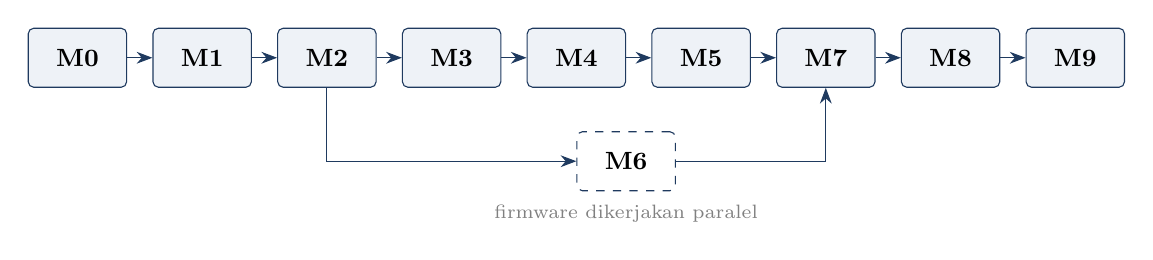
\begin{tikzpicture}[node distance=0.32cm,
  box/.style={draw=navy,fill=soft,rounded corners=2pt,minimum width=1.25cm,minimum height=0.75cm,font=\small\bfseries},
  par/.style={draw=navy,dashed,fill=white,rounded corners=2pt,minimum width=1.25cm,minimum height=0.75cm,font=\small\bfseries},
  ar/.style={-{Stealth[length=2mm]},navy}]
  \node[box] (m0) {M0};
  \node[box,right=of m0] (m1) {M1};
  \node[box,right=of m1] (m2) {M2};
  \node[box,right=of m2] (m3) {M3};
  \node[box,right=of m3] (m4) {M4};
  \node[box,right=of m4] (m5) {M5};
  \node[box,right=of m5] (m7) {M7};
  \node[box,right=of m7] (m8) {M8};
  \node[box,right=of m8] (m9) {M9};
  \node[par,below=0.55cm of m4.south east,anchor=north] (m6) {M6};
  \foreach \a/\b in {m0/m1,m1/m2,m2/m3,m3/m4,m4/m5,m5/m7,m7/m8,m8/m9} \draw[ar] (\a)--(\b);
  \draw[ar] (m2.south) |- (m6.west);
  \draw[ar] (m6.east) -| (m7.south);
  \node[font=\scriptsize,color=gray,below=0.05cm of m6] {firmware dikerjakan paralel};
\end{tikzpicture}
\end{center}

% ------------------------------------------------------------------ arsitektur
\clearpage
\section{Rekomendasi arsitektur}

\subsection{Sistem}

\begin{center}
\begin{tikzpicture}[node distance=0.55cm and 0.7cm,
  b/.style={draw=navy,fill=soft,rounded corners=2pt,align=center,font=\small,minimum height=0.9cm,text width=2.3cm},
  w/.style={draw=navy!60,fill=white,rounded corners=2pt,align=center,font=\small,minimum height=0.9cm,text width=2.3cm},
  ar/.style={-{Stealth[length=2mm]},navy},
  wa/.style={-{Stealth[length=2mm]},blue!60!black,thick}]
  % aliran air
  \node[w] (tank) {Tangki\\+ sekat};
  \node[w,right=of tank] (pump) {Pompa DC\\+ katup searah};
  \node[w,right=of pump] (s1) {S1\\(YF-S201)};
  \node[w,right=of s1] (ts) {Venturi\\+ tanjakan};
  \node[w,right=of ts] (gn) {Leher angsa\\+ corong};
  \draw[wa] (tank)--(pump); \draw[wa] (pump)--(s1); \draw[wa] (s1)--(ts); \draw[wa] (ts)--(gn);
  \draw[wa] (gn.south) -- ++(0,-0.45) -| (tank.south);
  \node[font=\scriptsize,color=blue!60!black,anchor=north west] at ($(tank.south)+(0.15,-0.5)$) {air balik (gravitasi)};
  % manometer
  \node[w,above=of ts] (mano) {Panel\\manometer};
  \draw[ar,dashed] (ts)--(mano);
  % elektronik
  \node[b,below=1.6cm of s1] (mcu) {ESP32-C3\\Super Mini};
  \node[b,left=of mcu] (drv) {Buck / MOSFET\\pompa};
  \node[b,right=of mcu] (ui) {LCD 20×4\\kenop, tombol};
  \node[b,below=of mcu] (pwr) {Adaptor 12 V\\sekring, buck 5 V};
  \draw[ar] (s1.south) -- node[right,font=\scriptsize]{pulsa (level shifter)} (mcu.north);
  \draw[ar] (mcu)--(drv); \draw[ar] (drv.north) -- (pump.south);
  \draw[ar,{Stealth[length=2mm]}-{Stealth[length=2mm]}] (mcu)--(ui);
  \draw[ar] (pwr)--(mcu);
\end{tikzpicture}
\end{center}

\textbf{Keputusan yang sudah dikunci (Rev.~08):} satu tangki + pompa langsung; leher angsa (tanpa servo); kenop target debit dengan kontrol PI; paket inti = zona A + B; MCU ESP32-C3 Super Mini; pompa MAXPUMP 12~V 19~W.

\subsection{Firmware}

Arsitektur \textbf{modul kecil + mesin keadaan (state machine)}. Tiap modul satu tanggung jawab, dan logika murni (tanpa akses hardware) dipisah supaya bisa diuji di laptop.

\begin{tabularx}{\linewidth}{@{}l L l@{}}
\toprule
\textbf{Modul} & \textbf{Tanggung jawab} & \textbf{Uji di laptop?} \\
\midrule
\texttt{flow} & Interrupt pulsa S1, ukur periode, konversi ke L/min pakai tabel faktor-K & Konversi: ya \\
\texttt{pi} & Kontrol PI dengan batas keluaran dan anti-windup & Ya \\
\texttt{pump} & Keluaran ke pompa (PWM atau buck), batas maksimum, default mati & Tidak \\
\texttt{safety} & Masa tenggang start, deteksi debit tak tercapai, watchdog & Ya \\
\texttt{physics} & v = Q/A, prediksi Δh, diameter leher terukur & Ya \\
\texttt{ui} & LCD, kenop, tombol (debounce), buzzer & Debounce: ya \\
\texttt{logger} & Baris CSV lewat serial & Format: ya \\
\texttt{config} & Konstanta: diameter, faktor-K, batas, pin & -- \\
\texttt{app} & Mesin keadaan, memanggil semua modul & Transisi: ya \\
\bottomrule
\end{tabularx}

\begin{center}
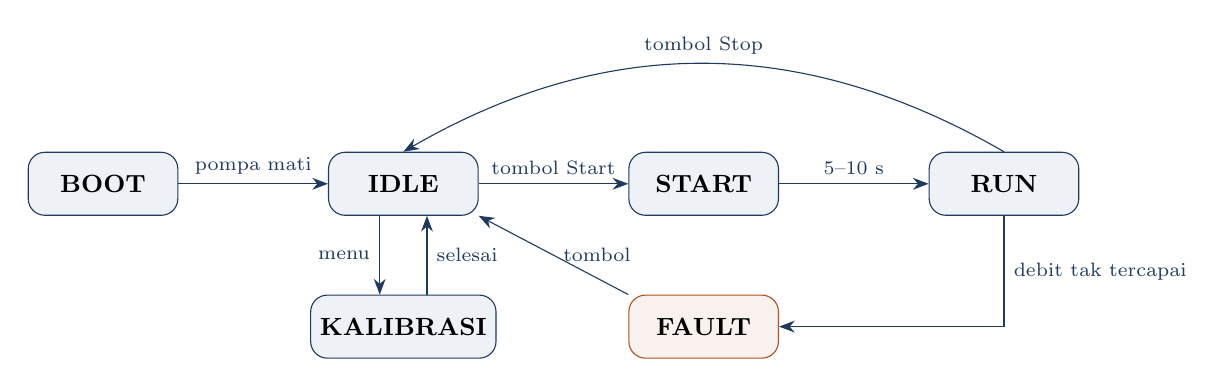
\begin{tikzpicture}[node distance=0.5cm and 1.9cm,
  st/.style={draw=navy,fill=soft,rounded corners=6pt,font=\small\bfseries,minimum width=1.9cm,minimum height=0.8cm},
  ft/.style={draw=warn,fill=warn!8,rounded corners=6pt,font=\small\bfseries,minimum width=1.9cm,minimum height=0.8cm},
  ar/.style={-{Stealth[length=2mm]},navy},
  lb/.style={font=\scriptsize,midway}]
  \node[st] (boot) {BOOT};
  \node[st,right=of boot] (idle) {IDLE};
  \node[st,right=of idle] (start) {START};
  \node[st,right=of start] (run) {RUN};
  \node[ft,below=1.0cm of start] (fault) {FAULT};
  \node[st,below=1.0cm of idle] (cal) {KALIBRASI};
  \draw[ar] (boot) -- node[lb,above]{pompa mati} (idle);
  \draw[ar] (idle) -- node[lb,above]{tombol Start} (start);
  \draw[ar] (start) -- node[lb,above]{5--10 s} (run);
  \draw[ar] (run.south) |- node[lb,right,pos=0.25]{debit tak tercapai} (fault.east);
  \draw[ar] (fault.north west) -- node[lb,right]{tombol} (idle.south east);
  \draw[ar] (run.north) to[bend right=30] node[lb,above]{tombol Stop} (idle.north);
  \draw[ar] ([xshift=-3mm]idle.south) -- node[lb,left]{menu} ([xshift=-3mm]cal.north);
  \draw[ar] ([xshift=3mm]cal.north) -- node[lb,right]{selesai} ([xshift=3mm]idle.south);
\end{tikzpicture}
\end{center}
{\small FAULT: pompa mati, layar menulis sebab dan cara restart, buzzer berbunyi. Kembali ke IDLE lewat tombol.}

\subsection{Struktur kode}

Gunakan \textbf{PlatformIO} (VS Code) dengan dua \emph{environment}: \texttt{esp32c3} untuk board dan \texttt{native} untuk unit test di laptop.

\begin{lstlisting}
firmware/
  platformio.ini        ; env:esp32c3 + env:native
  include/config.h      ; pin, diameter, batas, faktor-K
  src/
    main.cpp            ; setup() + loop() memanggil app
    app.cpp/.h          ; state machine
    flow.cpp/.h   pi.cpp/.h   pump.cpp/.h   safety.cpp/.h
    physics.cpp/.h   ui.cpp/.h   logger.cpp/.h
  test/
    test_pi/  test_flow/  test_safety/  test_physics/
\end{lstlisting}

\textbf{Aturan kode:} tidak ada \texttt{delay()} di loop utama (pakai \texttt{millis()}); semua konstanta di \texttt{config.h}; logika murni tidak memanggil fungsi Arduino; keluaran pompa selalu lewat \texttt{pump} yang memeriksa batas.

\subsection{Git}
\begin{itemize}
  \item Satu commit per perubahan yang utuh, pesan jelas (bahasa Indonesia).
  \item Tag tiap milestone selesai: \texttt{m1-uji-bangku}, \texttt{m4-fabrikasi}, \texttt{m7-kalibrasi}, \texttt{v1.0-serah-terima}.
  \item Hasil uji (foto, tabel) disimpan di \texttt{catatan/hasil-uji/}.
\end{itemize}

% ------------------------------------------------------------------ milestone
\section{Rincian milestone}

\ms{M0 — Kesepakatan dan kebutuhan skripsi}{2--4 hari}{Menentukan definisi ``selesai'' sebelum mengeluarkan uang.}
\begin{itemize}
  \item[\cek] Minta BAB I--III (minimal judul, rumusan masalah, metode).
  \item[\cek] Tentukan jenis skripsi: R\&D alat atau verifikasi eksperimen.
  \item[\cek] Client memilih paket inti atau lengkap.
  \item[\cek] Lengkapi dan kirim \texttt{catatan/draf-kesepakatan.md} + RAB.
  \item[\cek] Konfirmasi penghapusan servo dan bentuk interaksi (kenop debit).
  \item[\cek] Terima DP jasa + dana komponen tahap uji bangku.
\end{itemize}
\gate{kesepakatan disetujui tertulis, DP diterima, paket dan kriteria penerimaan jelas.}

\ms{M1 — Uji bangku}{3--5 hari}{Membuktikan asumsi desain dengan biaya kecil. Panduan: \texttt{catatan/uji-bangku.md}.}
\begin{itemize}
  \item[\cek] Beli: pompa, buck, adaptor, ESP32-C3, YF-S201, katup searah, level shifter, MOSFET, gelas ukur, jangka sorong.
  \item[\cek] Firmware uji (lihat M6 tahap 1): baca S1, atur keluaran pompa manual, log serial.
  \item[\cek] Ukur kurva tegangan → debit pompa, tegangan minimum stabil, head saat katup tertutup.
  \item[\cek] Kalibrasi awal S1 (gelas ukur, 5 ulangan per debit).
  \item[\cek] Uji katup searah (tahan 170 mm, 10 menit).
  \item[\cek] Ukur diameter dalam pipa riil; cetak 2--3 venturi, ukur leher, uji rembes.
\end{itemize}
\gate{4--6 L/min stabil, katup searah rapat, S1 terkalibrasi, diameter pipa dan leher terukur.}
{\small\color{warn}\textbf{Kalau gagal:} pompa tidak stabil di debit rendah → hambatan di hulu atau bypass (lihat \texttt{03-pompa.md}); katup searah bocor → ganti tipe; lalu ulangi M1.}

\ms{M2 — Desain final (Rev.~09)}{2--3 hari}{Mengganti angka asumsi dengan angka hasil uji.}
\begin{itemize}
  \item[\cek] Hitung ulang \texttt{01}--\texttt{03} dengan diameter dan kurva pompa riil.
  \item[\cek] Tentukan cara kendali pompa (PWM atau buck) dan batas keluaran.
  \item[\cek] Gambar ukuran rangka, panel, tangki (sketsa dengan dimensi).
  \item[\cek] Finalisasi RAB dengan harga riil; kirim selisih ke client bila ada.
\end{itemize}
\gate{semua kolom manometer masuk 0--350 mm pada rentang debit kerja; RAB final disetujui.}

\ms{M3 — Belanja komponen}{3--7 hari}{Membeli sisa komponen sesuai RAB final.}
\begin{itemize}
  \item[\cek] Isi kolom harga online, toko, status di RAB; simpan nota.
  \item[\cek] Periksa barang datang: ukuran, jumlah, tidak cacat.
  \item[\cek] Semua tabung manometer dari satu batch (diameter sama).
\end{itemize}
\gate{semua barang berstatus ``Diterima'' dan sesuai spesifikasi.}

\ms{M4 — Fabrikasi mekanik dan hidrolik}{4--6 hari}{Merakit badan alat dan jalur air.}
\begin{itemize}
  \item[\cek] Pelat dasar, rangka, panel manometer (skala 0--350~mm, garis merah z, skala kedua, peta pipa).
  \item[\cek] Tangki: bulkhead, sekat, saringan hisapan, keran kuras.
  \item[\cek] Jalur pipa: S1 → pipa lurus ≥ 20~cm → venturi → tanjakan → ball valve → leher angsa → corong.
  \item[\cek] Sadap tegak lurus dan bebas duri; selang, klem buang udara, peredam, talang limpah.
  \item[\cek] Datum: angka 0 skala sejajar sumbu pipa bawah (waterpass/selang air).
  \item[\cek] Uji bocor: terisi 24 jam.
\end{itemize}
\gate{tidak bocor 24 jam; uji nol (pompa mati) → semua kolom sama tinggi ± 1~mm.}

\ms{M5 — Elektronik}{2--3 hari}{Merakit rangkaian yang aman dekat air.}
\begin{itemize}
  \item[\cek] Rangkaian di PCB lubang: ESP32-C3, level shifter, MOSFET/buck, pull-down gate, filter sinyal S1.
  \item[\cek] Daya: adaptor 12~V → sekring → buck 5~V untuk MCU; jalur kabel pompa terpisah dari kabel sensor.
  \item[\cek] Kotak tahan cipratan di atas garis air; LCD, kenop, tombol di panel.
  \item[\cek] Uji tegangan tiap titik sebelum MCU dipasang.
\end{itemize}
\gate{pompa tidak menyala saat reset/upload; tidak ada pulsa palsu dari S1 saat pompa jalan.}

\ms{M6 — Firmware}{5--7 hari, paralel M4--M5}{Menulis kode bertahap, tiap tahap bisa dijalankan.}
\begin{enumerate}
  \item[\cek] \textbf{Tahap 1 (untuk M1):} \texttt{flow} + \texttt{pump} manual + \texttt{logger}.
  \item[\cek] \textbf{Tahap 2:} \texttt{pi} + \texttt{safety} + state machine (IDLE, START, RUN, FAULT).
  \item[\cek] \textbf{Tahap 3:} \texttt{ui} (LCD, kenop, tombol CEK, buzzer) + \texttt{physics}.
  \item[\cek] \textbf{Tahap 4:} mode KALIBRASI (input faktor-K), watchdog, rapikan, komentar seperlunya.
\end{enumerate}
\gate{semua unit test lulus; debit mengikuti target ± 3\% dalam 10 detik; FAULT terpicu saat katup ditutup.}

\ms{M7 — Integrasi, kalibrasi, uji terima}{3--4 hari}{Membuktikan alat memenuhi kriteria kesepakatan.}
\begin{itemize}
  \item[\cek] Kalibrasi akhir S1 di alat jadi; simpan faktor-K di firmware.
  \item[\cek] Ukur diameter leher final; masukkan ke \texttt{config.h}.
  \item[\cek] Jalankan uji terima (Bagian~\ref{sec:test}) dan isi tabel hasil.
  \item[\cek] Plot Δh terhadap Q² (≥ 5 debit): harus lurus lewat nol.
\end{itemize}
\gate{semua kriteria penerimaan di kesepakatan terpenuhi dan tercatat.}

\ms{M8 — Dokumentasi dan serah terima}{2 hari}{Client bisa memakai alat sendiri tanpa bertanya.}
\begin{itemize}
  \item[\cek] SOP: pengisian, buang udara, uji nol, menjalankan, mematikan, menguras.
  \item[\cek] Manual singkat + foto berlabel + diagram rangkaian.
  \item[\cek] Laporan kalibrasi (tabel faktor-K, C\textsubscript{d} terukur, plot Δh vs Q²).
  \item[\cek] Demo ke client; client mencoba sendiri satu siklus praktikum.
  \item[\cek] Tag \texttt{v1.0-serah-terima}; terima pelunasan.
\end{itemize}
\gate{berita acara serah terima ditandatangani.}

\ms{M9 — Garansi}{sesuai kesepakatan}{Menjaga alat tetap jalan selama pengambilan data skripsi.}
\begin{itemize}
  \item[\cek] Catat setiap keluhan dan perbaikan di \texttt{catatan/}.
  \item[\cek] Siapkan suku cadang: YF-S201 dan ESP32-C3 cadangan.
\end{itemize}

% ------------------------------------------------------------------ test
\section{Rencana pengujian}\label{sec:test}

\subsection{Unit test firmware (di laptop, \texttt{pio test -e native})}
\begin{tabularx}{\linewidth}{@{}l L@{}}
\toprule
\textbf{Modul} & \textbf{Kasus uji} \\
\midrule
\texttt{flow} & Periode pulsa → L/min benar; tanpa pulsa > 1 s → 0; interpolasi tabel faktor-K \\
\texttt{pi} & Keluaran naik saat debit < target; dibatasi maks; tidak \emph{windup} saat jenuh \\
\texttt{safety} & Tidak memicu FAULT selama masa tenggang; memicu setelah 3 s debit < 50\% target \\
\texttt{physics} & v dan prediksi Δh cocok dengan tabel di \texttt{02-profil-manometer.md} \\
\texttt{app} & Transisi state sesuai diagram; FAULT selalu mematikan pompa \\
\bottomrule
\end{tabularx}

\subsection{Uji hardware dan integrasi}
\begin{tabularx}{\linewidth}{@{}l L l@{}}
\toprule
\textbf{Uji} & \textbf{Cara} & \textbf{Milestone} \\
\midrule
Bocor & Isi air, diamkan 24 jam & M4 \\
Uji nol & Pompa mati, bandingkan semua kolom & M4, tiap sesi \\
Reset aman & Cabut-pasang daya dan upload ulang; amati pompa & M5 \\
Derau sensor & Pompa jalan, debit target 0; S1 harus 0 & M5 \\
Respon PI & Ubah target 4 → 6 L/min; catat waktu tunak & M6 \\
Pengaman & Tutup ball valve saat RUN; harus FAULT tanpa luapan & M6 \\
\bottomrule
\end{tabularx}

\subsection{Uji terima (kriteria kesepakatan)}
\begin{tabularx}{\linewidth}{@{}L l l@{}}
\toprule
\textbf{Kriteria} & \textbf{Target} & \textbf{Hasil} \\
\midrule
Debit stabil pada rentang kerja & 4--6 L/min & \\
S1 vs gelas ukur & ± 5\% & \\
Δh venturi vs prediksi (3 debit) & ± 10\% & \\
Uji nol & ± 1 mm & \\
Bocor 24 jam & tidak ada & \\
Δh vs Q² & lurus, lewat nol & \\
\bottomrule
\end{tabularx}

% ------------------------------------------------------------------ risiko
\section{Risiko utama}
\begin{tabularx}{\linewidth}{@{}L L l@{}}
\toprule
\textbf{Risiko} & \textbf{Penanganan} & \textbf{Dicek di} \\
\midrule
Budget client tidak cukup (RAB ± Rp4,2 jt vs Rp2 jt) & Kurangi scope di M0; jangan belanja sebelum sepakat & M0 \\
Pompa tersendat di debit rendah & Hambatan di hulu / bypass; atur lewat tegangan & M1 \\
Katup searah merembes & Ganti tipe swing berkualitas; SOP pancing ulang & M1 \\
Leher venturi meleset (Δh ∝ d\textsuperscript{-4}) & Cetak 2--3, ukur, pakai diameter terukur & M1, M7 \\
Manometer meluap & Talang limpah, batas keluaran, FAULT cepat & M4, M6 \\
Gelembung udara di selang & Air balik di balik sekat; buang udara tiap sesi & M4, M8 \\
Listrik dekat air & Kotak tahan cipratan di atas air, sekring, RCD lab & M5 \\
Lumut dan jentik & Kuras antarsesi; keran kuras & M8 \\
\bottomrule
\end{tabularx}

\end{document}
